\section{Methodology}
\label{sec:methodology}
We treat each relevant consumer-item as an individual object and shape them into weekly time series data
based on historical transactions. In this setup, target value at each time step (week) takes a binary input, 1/0 
(purchased/non purchased). \emph{Relevancy} of the consumer-item is defined by items transacted by consumer during training 
time window. \emph{Positive samples} (purchased/1) are weeks where consumer did transact for an item, whereas 
\emph{Negative samples} (non purchased/0) are the weeks where the consumer did not buy that item.
We apply sliding windows testing routine for generating
out of time results. The time series is split into 3 parts - train, validation and
test as shown in Table \ref{tab:datasplit}. All our models are built in a multi-object 
fashion, which allows the gradient movement to happen across all consumer-item combinations split in batches. This enables 
cross-learning to happen across consumers/items. We then perform Feature Engineering over data splits to generate
modelling features. Below are some of the feature groups we perform our experiments with:
\begin{itemize}
\item {\bf Datetime:} We use transactional metrics at various temporal cuts like week, month, etc.
Datetime related features capturing seasonality and trend are also generated.
\item {\bf Consumer-Item Profile:} We use transactional metrics at different granularities like consumer, item,
consumer-item, department and aisle. We also create features like Time since first order, 
Time since last order, time gap between orders, Reorder rates, Reorder frequency, 
Streak - user purchased the item in a row, Average position in the cart, Total number of orders.
\item {\bf Consumer-Item-Time Profile:} We use transactional metrics at the intersection of consumer, item and time.
We generate interactions capturing consumer behaviour towards items at a given time.
\item {\bf Lagged Offsets:} We use statistical rolling operations like mean, median, quantiles, variance, 
kurtosis and skewness over temporal regressors for different lag periods to generate offsets.
\end{itemize}
The model we need to build, thus, should learn to identify similarly behaving time series across latent
parameters, and take into account consumer and item variations in comparing different time series. A row 
in time series is represented by
  \begin{equation}
    \begin{array}{l}
      y\textsubscript{cit}  = f(i\textsubscript{t}, c\textsubscript{t},..,c\textsubscript{t-n}, ic\textsubscript{t}
      ,..,ic\textsubscript{t-n}, d\textsubscript{t},..,d\textsubscript{t-n})
    \end{array}
    \label{eqn:fx}
  \end{equation}
where y\textsubscript{cit} is purchase prediction for consumer 'c' for item ’i’ at time ’t’. 
i\textsubscript{t} denotes attributes of item ’i’ like category, department, brand, color, size, etc at time 't'. 
c\textsubscript{t} denotes attributes of consumer 'c' like age, sex and transactional attributes at time 't'. 
ic\textsubscript{t} denotes transactional attributes of consumer 'c'  towards item 'i' at time 't'. 
d\textsubscript{t} is derived from datetime to capture trend and seasonality at time 't'. 
'n' is the number of time lags.

\begin{table}[t]
\caption{Modelling data splits}
\vspace{0.5 in}
\centering
\resizebox{5.5in}{!}
{%
\begin{tabular}{|c|c|c|c|}
\hline
{\bf Data Split} & {\bf Specifications} & {\bf Consumer-Item combinations} & {\bf Max Time-Series length} \\  
\hline\hline
Train  		&  Model training &  50,872 &  46 weeks \\ \hline
Validation	  		&  HyperParameter Optimization &  50,888 &  2 weeks \\ \hline
Test	  		&  Reporting Accuracy Metrics & 50,910 &  2 weeks\\
\hline
\end{tabular}
}
\label{tab:datasplit}
\end{table}

\subsection{Modelling}
\subsubsection{Feature Engineering}
From data classification, Figure \ref{fig:dnndata}, we can see that data was sub-divided 4 groups:
\begin{itemize}
\item {\bf Static Categorical:} These are categorical features that do not vary with time. This includes consumer
attributes like sex, marital status and location along with different item attributes like category, department and brand.
\item {\bf Temporal Categorical:} These are categorical features that vary with time. It includes all the datetime 
related features like week, month of year, etc.
\item {\bf Static Continuous:} These features are static but continuous. This includes certain consumer attributes like
age and weight, item attributes like size, and certain derived features like target encoded features.
\item {\bf Temporal Continuous:} These are time varying continuous features. All consumer and item related
traditional attributes like number of orders, add to cart order, etc. falls under this bucket.
\end{itemize}
\subsubsection{Loss Function}
Since we are solving Binary Classification problem, we believe that Binary Cross-Entropy should be the most appropriate 
loss function for training the models. We use the below formula to calculate Binary Cross-Entropy:
  \begin{equation}
      \begin{array}{l}
        H\textsubscript{p} = - \frac{1}{N}$$\sum_{i=1}^{N}y.log(p(y))+
        (1- y).log(1-p(y))
      \end{array}
    \label{eqn:logloss}
  \end{equation}
here H\textsubscript{p} represents computed loss, y is the target value (label), and p(y) 
is the predicted probability against the target. The BCELoss takes non-negative values. We can infer 
from Equation \ref{eqn:logloss} that Lower the BCELoss, better the Accuracy.
\subsubsection{Model Architecture}
As mentioned earlier in this section, traditional machine learning models are not really a suitable choice for modelling \emph{f} 
(Equation \ref{eqn:fx}) due to non-linear interaction between the features.
We work with Temporal Convolution Network model as shown in Figure Figure \ref{fig:TCN}.
\begin{itemize}
\item {\bf Entity Embeddings + Temporal Convolutional Network:} TCN (Figure \ref{fig:TCN}), originally
proposed in \cite{lea2016temporal} , is considered a competitive architecture yielding the best results when evaluated over 
our experimental dataset. This network comprises of 3 dilated Convolutional networks combined with entity embeddings.
Similar to LSTM, this architecture, after convolving and concatenating flows into 
3 fully connected ReLU based layers yielding to dense layer which has sigmoid activation.
\end{itemize}
\begin{figure}[t]
    \centering 
    \caption{Data classification for DNN Architectures} 
    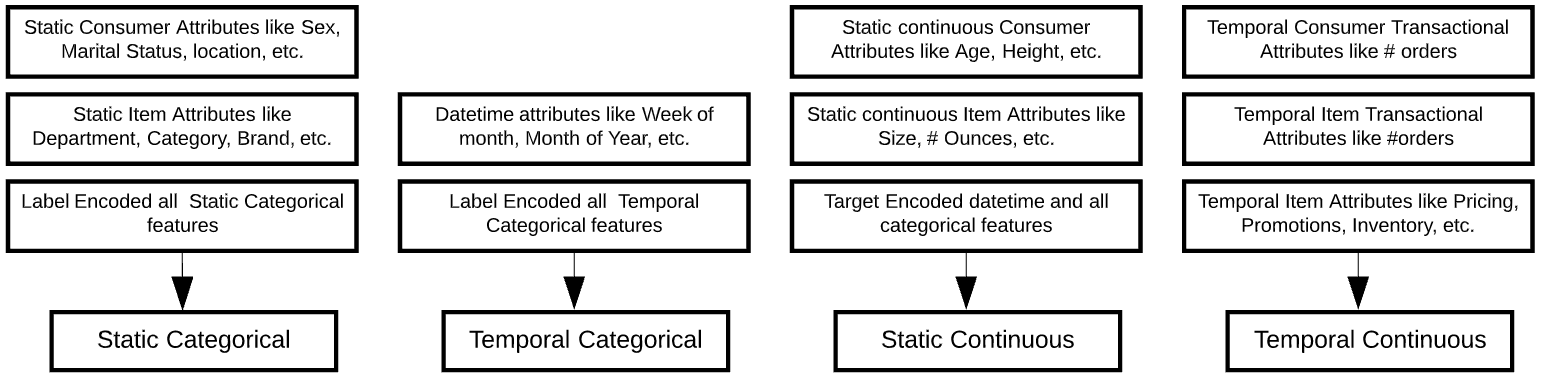
\includegraphics[width=5.5in]{img/dnndata.png} 
    \label{fig:dnndata} 
  \end{figure}
  \begin{figure}[t]
    \centering 
    \caption{Temporal Convolutional Network (TCN)} 
    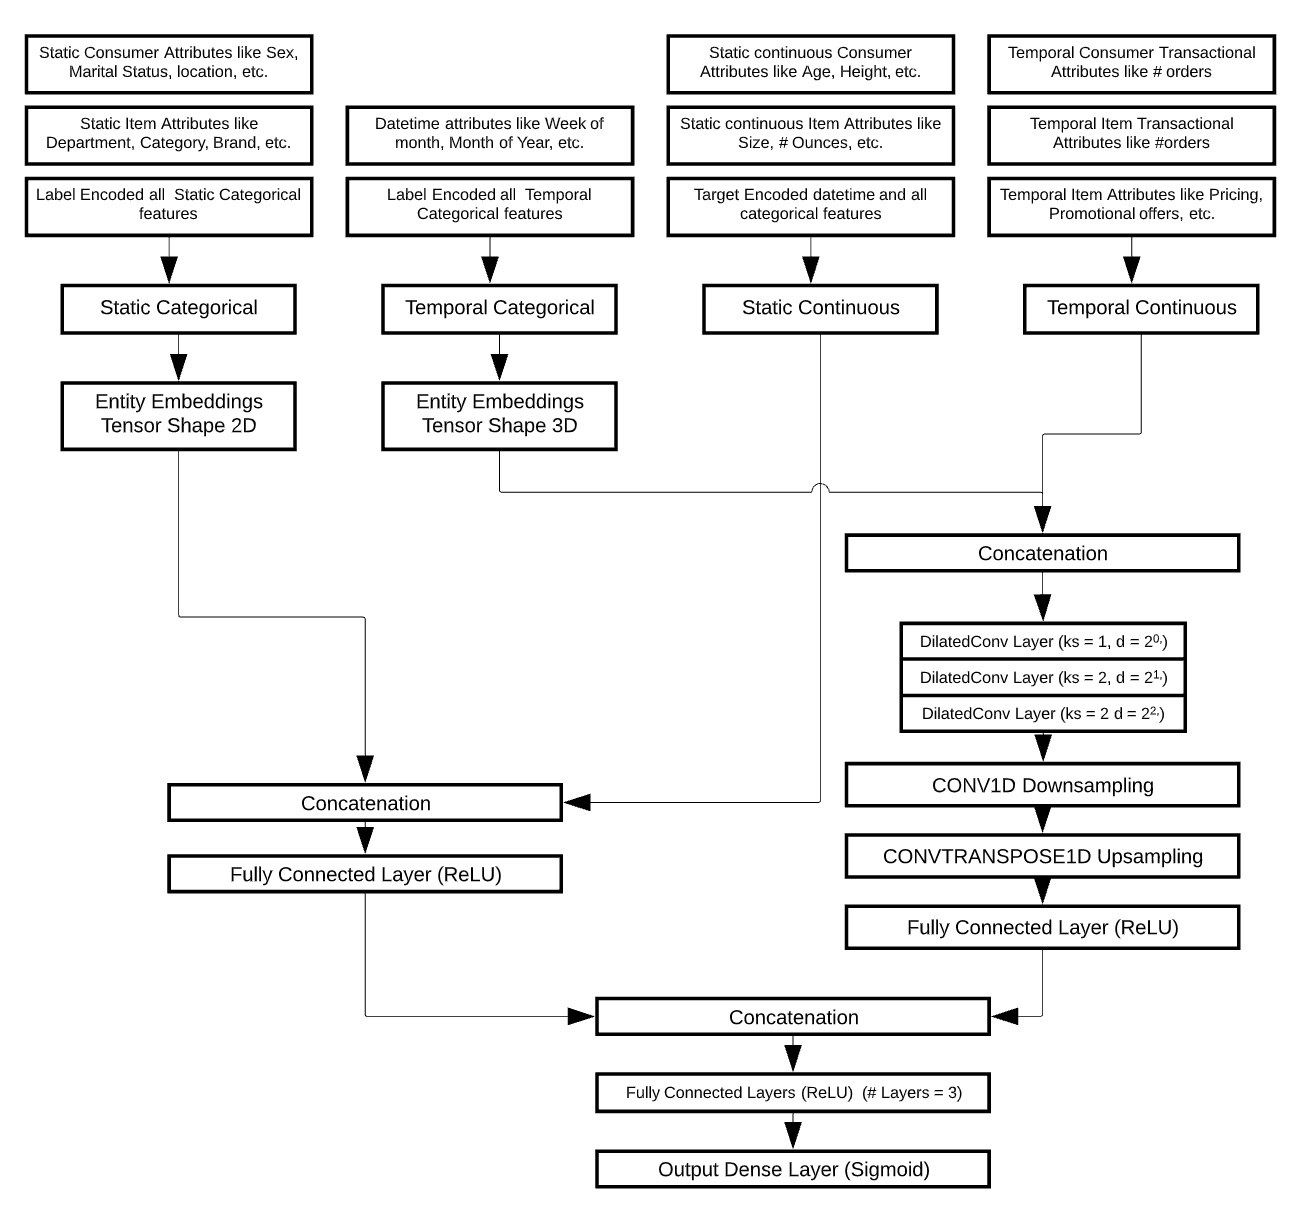
\includegraphics[width=5.5in]{img/TCN.png} 
    \label{fig:TCN} 
  \end{figure}
\subsubsection{Hyperparameter Tuning}
Hyper-parameters of tree based models are optimized
using Bayesian Hyperparameter Optimization Technique, Hyperopt \cite{bergstra2013hyperopt}. 
For Deep learning, we use documented best practices along with our experimental results to
choose model hyperparameters. Hyperparameter Optimization is performed over validation dataset. 
We list some of the hyperparameters along with the values we tune for Deep learning models.
  \begin{itemize}
    \item {\bf Optimizer Parameters:} RMSProp \cite{bengio2015rmsprop} and Adam are used as different trial configurations. 
    The learning rate is experimentally tuned to 1e-3. We also have weight decay of 1e-5 which helps a bit in model Regularization.
    \item {\bf Scheduler Parameters:} CyclicLR \cite{smith2017cyclical} and ReduceLROnPlateau \cite{zaheer2018adaptive} 
    Learning rates are used as different trial configurations.
    we use 1e-3 as max lr and 1e-6 as base lr for cyclical learning rate along with the step size being the function of
    length of train loader. ReduceLROnPlateau is tuned at 1e-6 as min lr.
    \item {\bf SWA:} Stochastic Weight Averaging (SWA) \cite{izmailov2018averaging} is used to improve generalization across Deep Learning
    models. SWA performs an equal average of the weights traversed by SGD with a modified learning rate schedule. We use 
    1e-3 as SWA learning rate.
    \item {\bf Parameter Average:} This is a method to average the neural network parameters of n best model checkpoints 
    post training, weighted by validation loss of respective checkpoints. The resulting model generalizes better than those 
    with a single best checkpoint model for an unseen data. 
  \end{itemize}
Apart from the above parameters we also iterate to tune network parameters like number of epochs, batch size, 
number of Fully Connected Layers, number of LSTM layers, convnet parameters (kernel size, dilations, padding)
and embedding sizes for the categorical features. Binary Cross-Entropy \ref{eqn:logloss} is used as loss 
function for all the models.
\subsection{F\textsubscript{1}-Maximization}
Post stacking, we optimize for purchase probability threshold based on
probability distribution at a consumer level using F\textsubscript{1}-Maximization.
This enables optimal thresholding of consumer level probabilities to  maximize F\textsubscript{1} measure \cite{lipton2014optimal}.
To illustrate the above, let us say we generated purchase probabilities for 
'n' items out of 'b' actually purchased items by consumer 'c'. Now, let us visualize the actuals (\ref{eqn:A}) 
and predictions (\ref{eqn:P})  of 'n' predicted items for consumer 'c'.
  \begin{equation}
    \begin{array}{l}
      A\textsubscript{c} = [a\textsubscript{1}, a\textsubscript{2}, .., a\textsubscript{n}] 
       \; \forall \; a\textsubscript{j} \in \; $\{0,1\}$
    \end{array}
    \label{eqn:A}
  \end{equation}
  \begin{equation}
    \begin{array}{l}
      P\textsubscript{c} = [p\textsubscript{1}, p\textsubscript{2}, .., p\textsubscript{n}]
      \; \forall \; p\textsubscript{j} \in \; [0,1]
    \end{array}
    \label{eqn:P}
  \end{equation}
A\textsubscript{c} represents the actuals for consumer 'c', with a\textsubscript{j} being 1/0 
(purchased/non purchased). P\textsubscript{c} represents the predictions 
for consumer 'c' for the respective item, with p\textsubscript{j} being probability value. 
'n' represents total items for which the model generated purchase probabilities for consumer 'c'.
Now we apply Decision rule D() which converts probabilities to binary predictions, as described below 
in Equation \ref{eqn:Decision}.
  \begin{equation}
    \begin{array}{l}
      D(Pr\textsubscript{c}) : P\textsubscript{c}\textsuperscript{1 x n}
      \to P\textsuperscript{'}\textsubscript{c}\textsuperscript{1 x n}
      \;\; : p\textsuperscript{'}\textsubscript{j} = 
        \begin{cases}
          1 & p\textsubscript{j} \geq Pr\textsubscript{c} \\
          0 & \text{Otherwise}
        \end{cases}
    \end{array}
    \label{eqn:Decision}
  \end{equation}
  \begin{equation}
    \begin{array}{l}
      P\textsuperscript{'}\textsubscript{c} = [p\textsuperscript{'}\textsubscript{1}, 
      p\textsuperscript{'}\textsubscript{2}, .., p\textsuperscript{'}\textsubscript{n}]\; 
      \forall \; p\textsuperscript{'}\textsubscript{j} \in \; $\{0,1\}$
    \end{array}
    \label{eqn:Pdash}
  \end{equation}
  \begin{equation}
    \begin{array}{l}
      k =\sum_{i=1}^{n}p\textsuperscript{'}\textsubscript{i}
    \end{array}
    \label{eqn:Pdash}
  \end{equation}
Pr\textsubscript{c} is the probability cut-off to be optimized for maximizing F\textsubscript{1} measure \cite{lipton2014optimal} 
for consumer 'c'. Decision rule D() converts probabilities P\textsubscript{c} to binary predictions 
P\textsuperscript{'}\textsubscript{c} such that if p\textsubscript{j} is less than 
Pr\textsubscript{c} then p\textsuperscript{'}\textsubscript{j} equals 0, otherwise 1.
'k' is the sum of predictions generated post applying Decision rule D(). Now we solve for F\textsubscript{1} measure
using equations and formulae described below.
  \begin{equation}
    \begin{array}{l}
      V\textsubscript{Pr\textsubscript{c}} = 
      P\textsuperscript{'}\textsubscript{c}
      \;\times\; A\textsubscript{c}\textsuperscript{T}
      \;
      \Rightarrow	
      \left( \begin{array}{ccc}
      p\textsuperscript{'}\textsubscript{1} & .. & 
      p\textsuperscript{'}\textsubscript{n}
      \end{array} \right)
      \times
      %
      \left( \begin{array}{ccc}
      a\textsubscript{1} \\
      .. \\
      a\textsubscript{n} \\
      \end{array} \right)
    \end{array}
    \label{eqn:probability}
  \end{equation}
  \begin{equation}
    \begin{array}{l}
      Precision\textsubscript{c}= \frac{V\textsubscript{Pr\textsubscript{c}}} {k}
      \;\;\;\;\;and\;\;\;\;
      Recall\textsubscript{c}= \frac{V\textsubscript{Pr\textsubscript{c}}} {b}
    \end{array}
    \label{eqn:F1}
  \end{equation}
  \begin{equation}
    \begin{array}{l}
      F\textsubscript{1\textsubscript{c}} = \frac{2 \times Precision\textsubscript{c} 
      \times Recall\textsubscript{c}} 
      {Precision\textsubscript{c} + Recall\textsubscript{c}}
      \;
      \;\;\;\;\Rightarrow	\;\;\;\;
      2 * 
      \frac{
        V\textsubscript{Pr\textsubscript{c}}
      }
      {
        k + b
      }
    \end{array}
    \label{eqn:Optimizer}
  \end{equation}
V\textsubscript{Pr\textsubscript{c}} represents the number of items with purchase 
probabilities greater than Pr\textsubscript{c} which were actually purchased (True Positives). 
As can be seen, Formulae \ref{eqn:F1} and \ref{eqn:Optimizer} are used to calculate Precision, Recall and 
F\textsubscript{1}-score for consumer 'c'. 
  \begin{equation}
    \max_{V\textsubscript{Pr\textsubscript{c}}} \;\;\;\; 2 * \frac{ V\textsubscript{Pr\textsubscript{c}}}{k + b}
    \;\;\;\;,\;\;\;\;  \text{subject to: } \;\;\;\;  Pr\textsubscript{c}  \in \; [0,1]
    \label{eq:constraint}
  \end{equation}
Equation \ref{eq:constraint} represents the optimization function we solve to generate purchase predictions (1/0) for each consumer.

\subsection{Elasticity Framework}
Elasticity estimate is arrived at using simulations. To achieve that, for each consumer-item combination, base 
offer percent is identified using the following criteria in order:
\begin{itemize}
\item Average of last 4 weeks non-zero offer percent values of the consumer-item combination
\item Average of historical non-zero offer percent values of the consumer-item combination
\item Average of last 4 weeks non-zero offer percent values of all same age consumer-item combinations within that category
\end{itemize}

  \begin{figure}[t]
    \centering 
    \caption{Purchase probability vs. Offer percentage} 
    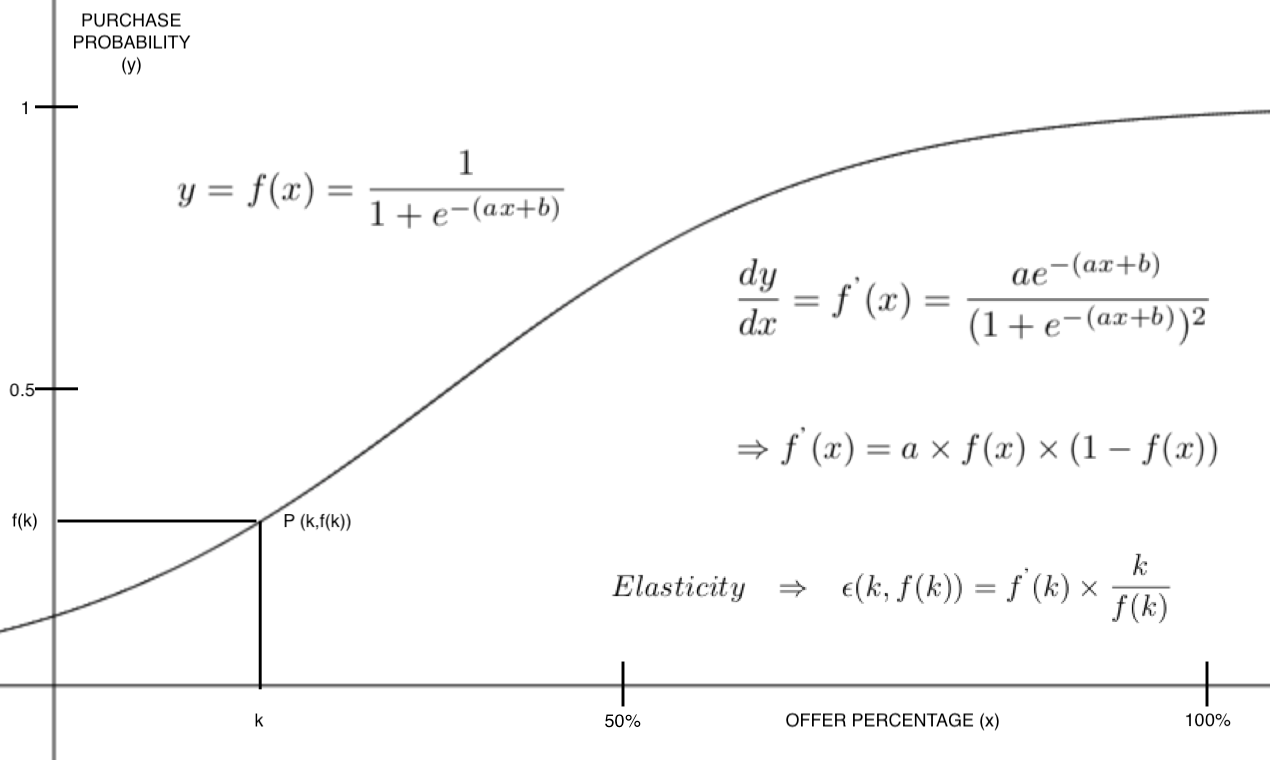
\includegraphics[width=4.4in]{img/elasticity.png} 
    \label{fig:elasticity} 
  \end{figure}
 
 \begin{equation}
    f(x) = \frac{1}{1 + e^{-(ax+b)}} \;\;\;\; ,\;\;\;\;
    f\textsuperscript{'}(x) = a\times f(x)\times (1 - f(x))
    \label{eq:fx}
  \end{equation}


 \begin{equation}
    \epsilon(k,f(k)) = f\textsuperscript{'}(k) \times\frac{k}{f(k)} \;\;\;\; \;\;\;\;
    \Rightarrow \epsilon(k,f(k)) = a\times k\times (1 - f(k))
    \label{eq:fx}
  \end{equation}

\subsection{Multi-Objective Optimization}
The optimization function needs to solve for the below Objectives:
\begin{itemize}
\item Maximize the Net Revenue (R\textsubscript{v})
\item Maximize the Retention rate (R\textsubscript{r})
\end{itemize}

 \begin{equation}
    R\textsubscript{v} = \sum_{i=1}^{n}\;\;\;[I\textsubscript{p} - \frac{I\textsubscript{p}}{100} \times (k \mypm \eta\times k)]
    \times
    \ \mathds{1} \ \textsubscript{c}(f(k) \mypm \eta\times \epsilon(k,f(k))\times f(k))
    \label{eq:fx}
  \end{equation}

\begin{equation}
    R\textsubscript{r} = \frac{\sum_{i=1}^{n}\; \ \mathds{1} \ \textsubscript{c}(f(k) \mypm \eta\times 
    \epsilon(k,f(k))\times f(k))}{n}
    \label{eq:fx}
  \end{equation}

  \begin{equation}
    \ \mathds{1} \ \textsubscript{c}(x) :=
        \begin{cases}
          1 & x \geq c\\
          0 & \text{Otherwise}
        \end{cases}
    \label{eq:fx}
  \end{equation}

Net Revenue (R\textsubscript{v}) will be a function of 

\begin{equation}
\begin{aligned}
\max_{\eta, \lambda, \gamma} \quad & 
\lambda R\textsubscript{v} + \gamma R\textsubscript{r}\\
\textrm{s.t.} \quad & 
\eta, \lambda, \gamma \in \; (0,1) \\
&\lambda + \gamma = 1\\
&R\textsubscript{r} >= R\textsubscript{rc} \\
\end{aligned}
\end{equation}

  \begin{figure}[t]
    \centering 
    \caption{Category wise Sales Distribution} 
    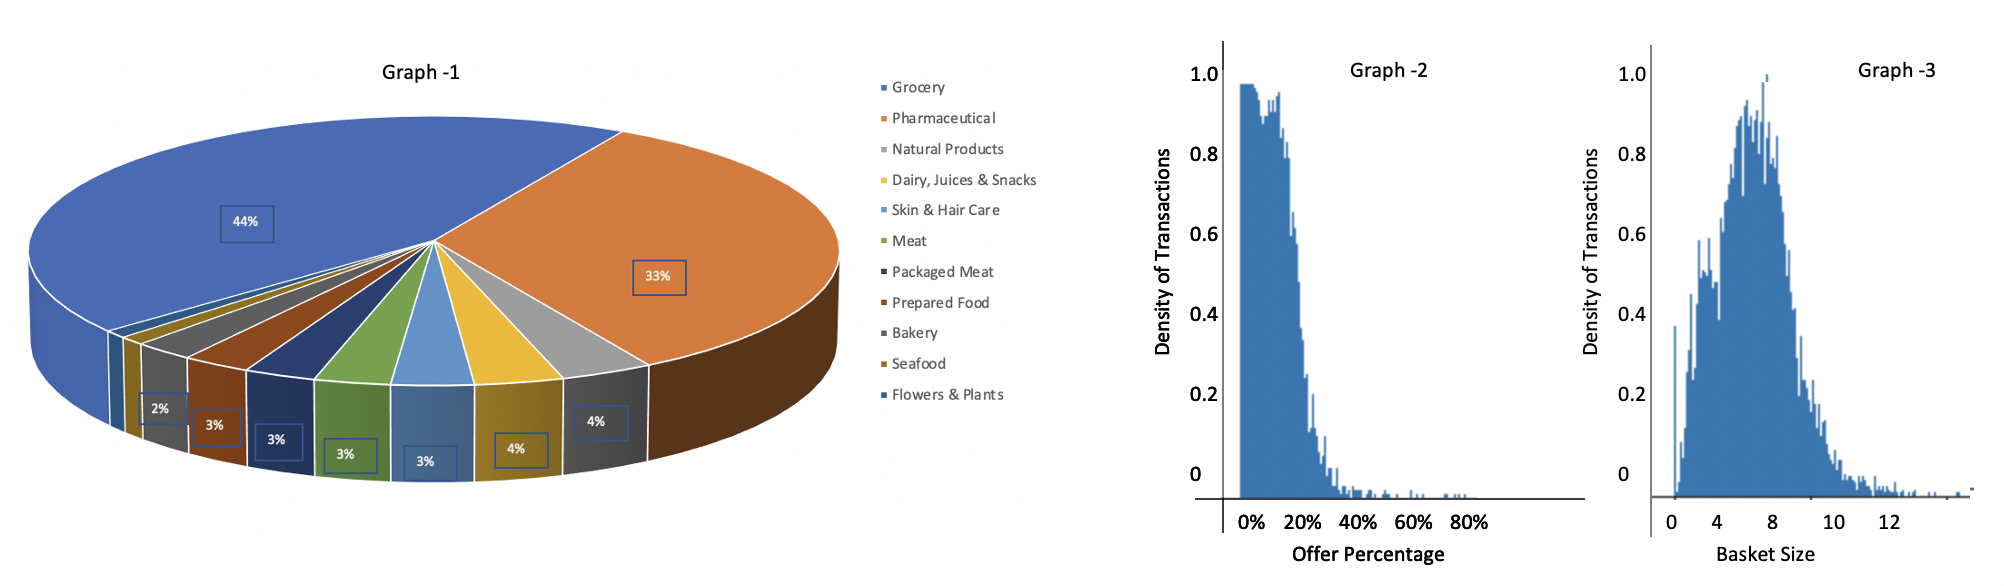
\includegraphics[width=5.5in]{img/sales_dist.png} 
    \label{fig:sales_dist} 
  \end{figure}

  \begin{figure}[t]
    \centering 
    \caption{Category graphs} 
    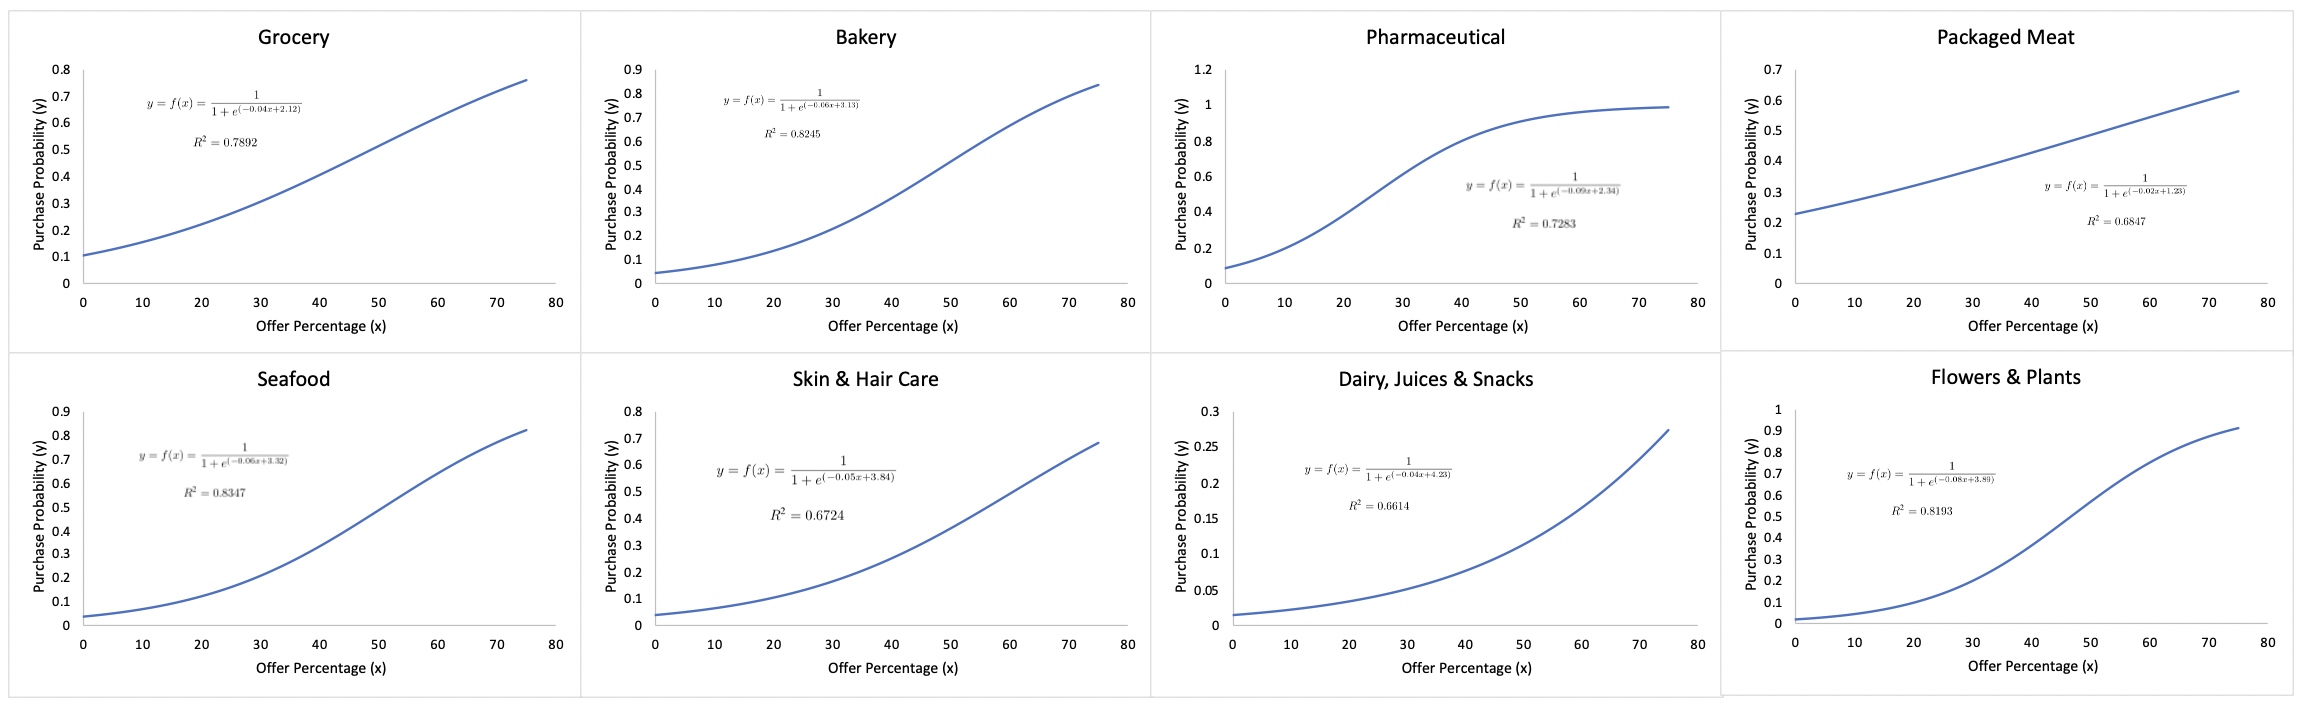
\includegraphics[width=5.5in]{img/cat_curves.png} 
    \label{fig:cat_curves} 
  \end{figure}

 \begin{figure}[t]
    \centering 
    \caption{Probability Distributions} 
    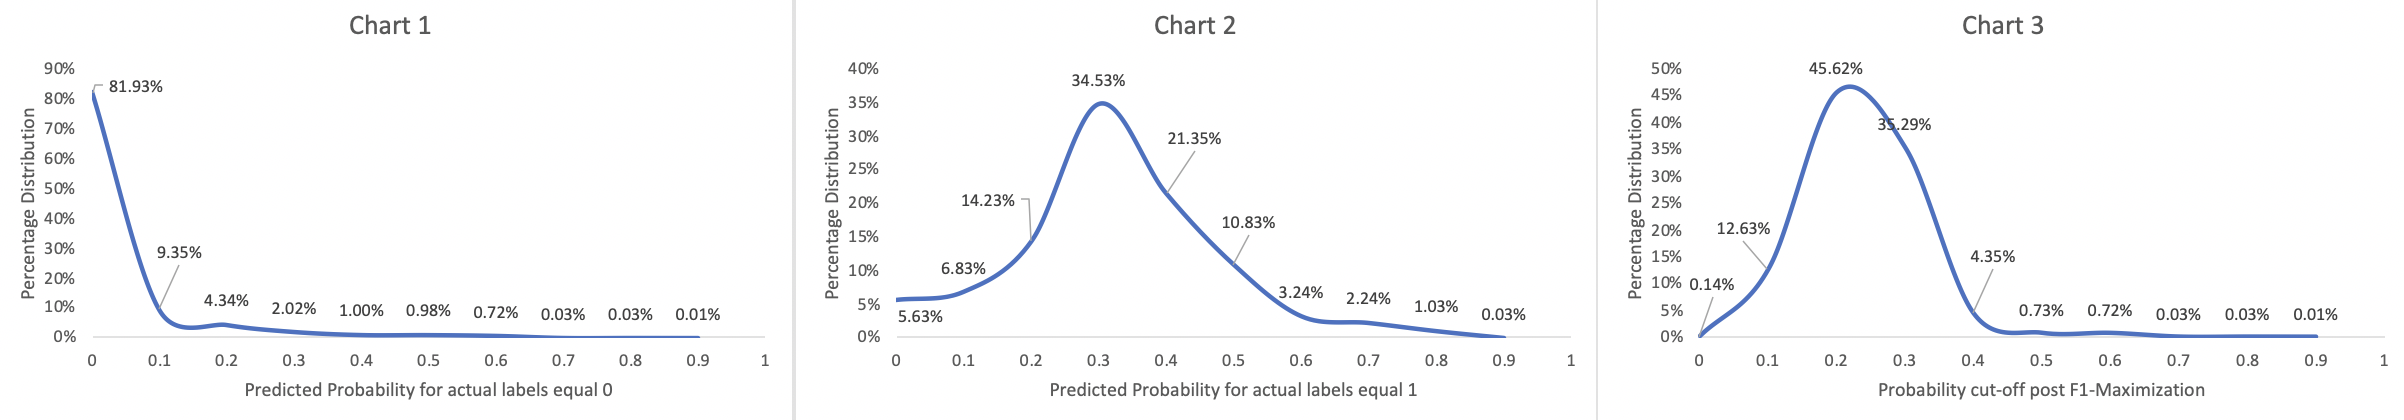
\includegraphics[width=5.5in]{img/prob_dist.png} 
    \label{fig:prob_dist} 
  \end{figure}
  
\begin{table}[t]
\caption{Modelling Results}
\vspace{0.3 in}
\centering
\resizebox{2.2in}{!}
{%
\begin{tabular}{|c|c|c|c|}
\hline
{\bf Metric} & {\bf Train} & {\bf Validation} & {\bf Test} \\  
\hline\hline
BCELoss  		&  0.0298 &  0.0318 &  0.0302 \\ \hline
Precision	  		&  0.512 &  0.489 &  0.508 \\ \hline
Recall	  		&  0.536 & 0.513&  0.523\\ \hline
F\textsubscript{1}-Score	&  0.523 & 0.501 &  0.515\\
\hline
\end{tabular}
}
\label{tab:datasplit}
\end{table}